\documentclass[authoryear, 12pt,5p, times]{elsarticle}
%\usepackage[hypcap]{caption}
%\geometry{margin=0.95in,top=1.4in,bottom=1.4in}
\geometry{margin=1in,top=1.3in,bottom=1.3in}
\usepackage{float}
\usepackage{amsmath}
\usepackage[hidelinks]{hyperref} 
 \usepackage{gensymb}
\usepackage{subcaption}
\usepackage{url}
%\renewcommand\thefootnote{\fnsymbol{\dagger}}
\usepackage[symbol*]{footmisc}
\newcommand{\rpm}{\raisebox{.2ex}{$\scriptstyle\pm$}}
\begin{document}
%\footnote{This is a footnote}
\begin{frontmatter}
\title{Asteroid Astrometry from CCD Images}
\author{\today \\ \quad \\Jung Lin (Doris) Lee\\ dorislee@berkeley.edu\\Group partners: Jennifer Ito, Manuel Silvia\\Prof. James Graham, UGSI Heechan Yuk, Isaac Domagalski}
	\begin{abstract}
astrometry for asteroid name..etc
	\end{abstract}
\end{frontmatter}
\section{Introduction}

\section{Data Reduction}
	
	\subsection{Systematic  Corrections}
The purpose of bias,dark, flat correction is to make the intensity of the image approximately linearly proportional to the number of astronomical photons arriving at the detector.
\paragraph{\textbf{Bias subtraction}}
Bias frames are images taken with zero integration time and used to subtract the digital offset at zero level. Common practice include taking a scalar value representative of the bias frame dataset (i.e. mean or median) and subtracting that from the original image. For the simple averaging method, the more bias frames we have the better, since as the number of bias frames we have increase, the standard deviation of the mean falls off as 1/$\sqrt{N}$, thereby decreasing the uncertainty on the obtained mean value.  We applied the method of indiscriminate rejection described by Chromey (2010) which removes the largest pixel value of the bias frame, then take the median on the remaining values. This method rejects the largest statistical outlier which is included when we simply take the mean for correction. Another method of bias correction is to set extra clock cycles so that the CCD reading continues for an additional 32 pixels after the physical image has been read out. Such  use of overscan pixels can be advantageous over bias frames for bias correction in the case when the bias is changing over time since each image has its own bias correction taken immediately after the exposure. We corrected an image by taking the median of the 32 pixel. The median is chosen over the mean so that anomalies such as cosmic ray events or nearby radio activity are rejected. Even though we experimented with all the methods described above, since the goal of this lab is to conduct astrometric measurements using these images rather than detailed photometric study,  we have simply chosen the more computationally trivial method of bias frame subtraction to apply to every image. 			
		\paragraph{\textbf{Dark and Flat Correction}}
	Dark frames are long-exposure images taken with the shutters closed to calibrate for dark responses. We conduct dark correction by subtracting from a single dark frame with  exposure time of 300 seconds. Since the CCD for Nickel Telescope is cooled by the LN2 dewar to a relatively low temperature, the thermal production of electrons is much lower than in room temperature. Therefore dark frames will not significantly improve the data quality. We took the dark and flat frames for the I,R filters taken on October 16, 2013  and applied them to the other data on the other days since dark and flat frames were not taken for the observation at the other dates. Using the twilight sky as a source of uniform illumination, the flat field images calibrate the pixel-by-pixel variation of each pixel. The exposure time was short and adjusted for every frame to accommodate for the sky's changing brightness. Every pixel on the 1024-by-1024 image is processed by : 
			\begin{equation}
			\frac{\text{image}-\text{dark}}{\text{flat}}\times\text{median(flat)}
			\end{equation}
		 As shown in the equation, we first dark-subtract from the image so that the intensity is linearly proportional to the number of photon counts then we divide by the flat in order to scale for the pixel-by-pixel variations. By plotting the pixel histogram of the image, we see that most of the pixel values are very small relative to our original image data at around 0.005 (@@@@UNITSSS). In order to preserve the comprehensible data ranges of the original intensity values after subtraction,  the image is normalized by a scalar value that is representative of the magnitude of the flat field data. The median value is chosen because unlike the mean its value is not skewed due to the bad pixel and columns present on the Nickel Telescope.

	\begin{figure}[h!]
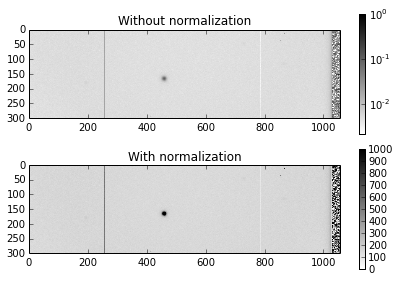
\includegraphics[width=0.5\textwidth]{figures/normalization}
\caption{Without normalization, the image requires a logarithmic stretch to distinguish the asteroid and the background since it has to accommodate for the range of decimal values resulted from the division. With normalization, the image can be viewed on a linear scale with a lower intensity limit of 0 and upper limit of 1000.}
\label{normalization}
\end{figure}
\subsection{Centroid-finding}
In order to determine the positions of the stars on the image, we need to find the centroid position with the weight as the 
First, we set a threshold which was empirically adjusted to yield just enough stars for pattern recognition at around 5000 (UNITSS!!!!). This identifies 
Since bad columns, corners, and borders often show up as completely dark pixels \footnote{Since image color scheme is inverted, the darkest pixel mean highest intensity.}, it is mistaken as a whole row of stars , we have to manually mask the pixels by zeroing the intensity value at the selected pixel.
	\begin{figure}[h!]
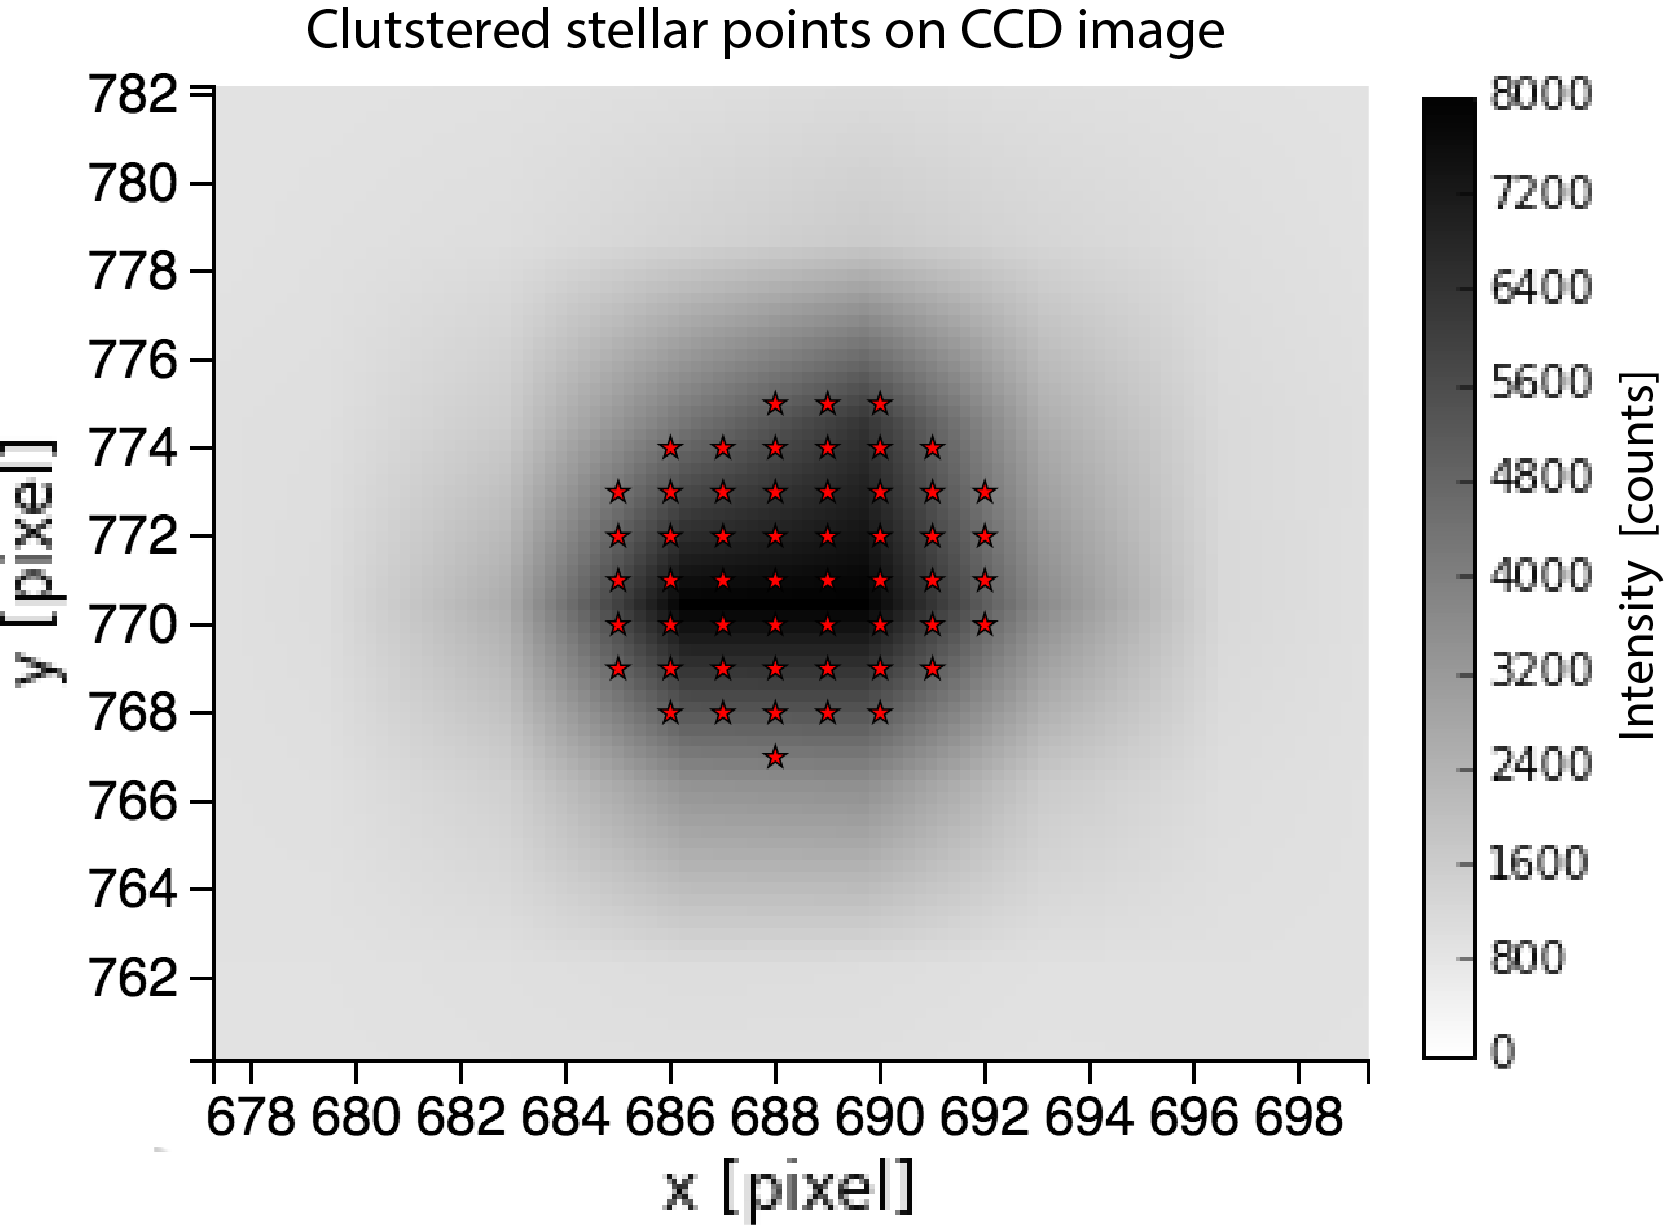
\includegraphics[width=0.5\textwidth]{figures/centroid_many}
\caption{CENTROID MANY STUFF}
\label{centroid_many}
\end{figure}
Since this is a fairly trivial case where the datapoints for each cluster is far apart, we use the more conceptually simplistic but computational intensive method of distance estimation instead of other clustering algorithm  in the literature.  We loop through list of points above the threshold and for every \_ we compute its pixel distance from another point in the same list. If the separation distance between two datapoints is smaller than 20 pixel, then it is clustered into the same star. Each cluster represent a star. This threshold radius is selected  \_ , most star have approx same aperture/ size because \_. Finally, in order to get a representative value from cluster information, we calculate the centroid by Eq. \ref{centroid_eq} :
\begin{equation}
x = \frac{\sum \limits_{i} x_i I_i}{\sum\limits_{i} I_i}
\label{centroid_eq}
\end{equation}

Error on centroid. 
\subsection{Pixel to Standard Coordinate conversion}
Since most stars used for (?) comparison are often very far away, it is convientent to treat them as projected position onto a sphere centered at the observer.
\section{Astrometry}
Using stellar positions to calibrate the image
	\subsection{Centroid Finding}
		\subsubsection{Algorithm}
	\subsection{Least Square}
	The purpose of using the least square method is to find a conversion matrix between the CCD-based pixel coordinate to standard coordinate.
	The standard coordinates can then be projected to celestial coordinates based on the Eq. (LABEL!!!):
	(TYPE EQUATION HERE)
	\subsubsection{USNO}
	intentionally adjust the Vmag lower cut than Vmag observed in NASA's small object dynamic so that it is able to identify the asteroid as a star.
	\subsection{Ephemeris information}	
Position vector can be obtained from the HORIZONS Web-Interface 
heliocentric vector to Earth
This could be verified with the vector from earth to asteroid.
	JPL horizon by default returns the ecliptic coordinate, Make sure to chose equtorial coordinate . This would affect the values for y and z components of the position (and velocity) vector returned since in the equitorial system the plane is around the equator
	
	 xy-plane: plane of the Earth's mean equator at the reference epoch
    x-axis  : out along ascending node of instantaneous plane of the Earth's
              orbit and the Earth's mean equator at the reference epoch
    z-axis  : along the Earth mean north pole at the reference epoch
    
\section{Conclusion}

 \section{References}
%\bibliographystyle{elsarticle-harv}
\begin{itemize}
\item Howell, Steve,  \textit{Handbook of CCD Astronomy}, 2nd Edition. Cambridge University Press, 2006.
\item Wall, J. V. and Jenkins, C.R., \textit{Practical Statistics for Astronomers}, Cambridge University Press, 2002.
\item Press, William H., and William T. Vetterling. \textit{Numerical Recipes in C: The Art of Scientific Computing}. Cambridge University Press, 1992. 
\end{itemize}
\end{document}
